% !TEX root = ../HonoursThesis.tex

\renewcommand{\chapterlabel}{Chapter}
\chapter{Echo state network with ordinal partition based sub-reservoirs}
\label{chap:OPESNs}


The second proposal uses a restricted reservoir and routed input to structurally encode the information given by ordinal partitioning of the data into the model. We will call this model an `Ordinal Partition Echo State Network' or OPESN. The reservoir consists of $N_{obs}$ sub-reservoirs of size $k$, where $N_{obs}$ is the number of non-forbidden ordinal partitions of the training sequence. In the primary case, the sub-reservoirs are connected `one-to-one', with one node of each sub-reservoir possibly connected to one node of each other sub-reservoir. The connections from one sub-reservoir to another sub-reservoir are scaled according to the probability of transitioning between them. We also test multiple other schemes for connecting the sub-reservoirs.

An input is routed to the relevant sub-reservoir depending on the ordinal partition of the observation. If an input observation is from ordinal partition `3' then it will be used to update the states of sub-reservoir `3' and an input value of 0 will be used to update the states of the other sub-reservoirs. We will refer to the sub-reservoir to which input is routed at any time step as the `active sub-reservoir'. Figure \ref{fig:OPESN} provides a diagram of the OPESN.

\begin{figure}
        
    \centering
    \begin{tikzpicture}%[scale=0.8]
        \node[fill=col1,circle,inner sep=4pt,label=left:$\mathbf{x}(t)$] (input) at (0,0) {};
        \node[fill=black,circle,inner sep=2pt,label=right:$\mathbf{y}(t)$] (output) at (10,0) {};
        


        % Layer 1
        
        % The nodes of the reservoir
        \coordinate (res_anchor) at (5,3);
        \node[fill=black,circle,inner sep=2pt] (res1) at ($(res_anchor) + (-0.5,0.8)$) {};
        \node[fill=black,circle,inner sep=2pt] (res2) at ($(res_anchor) + (0,-1)$) {};
        \node[fill=black,circle,inner sep=2pt] (res3) at ($(res_anchor) + (0,0.15)$) {};
        \node[fill=black,circle,inner sep=2pt] (res4) at ($(res_anchor) + (1,-0.1)$) {};
        \node[fill=black,circle,inner sep=2pt] (res5) at ($(res_anchor) + (-0.75,-0.5)$) {};
        \node[fill=black,circle,inner sep=2pt] (res6) at ($(res_anchor) + (-1.25,0.4)$) {};
        \node[fill=black,circle,inner sep=2pt] (res7) at ($(res_anchor) + (0.65,0.75)$) {};
        \node[fill=black,circle,inner sep=2pt] (res8) at ($(res_anchor) + (1,-0.9)$) {};
        \node[fill=black,circle,inner sep=2pt] (res9) at ($(res_anchor) + (-1.25,-1)$) {};
        \node[fill=black,circle,inner sep=2pt] (res10) at ($(res_anchor) + (-1.75,-0.25)$) {};
        
        % The internal connections in the reservoir
        \foreach \i in {1,...,5}
            \foreach \j in {1,...,5} {
                \ifnum\i<\j
                    \draw (res\i) -- (res\j);
                \fi
            }
        
        % More internal connections in the reservoir
        \draw (res6) -- (res5);
        \draw (res6) -- (res1);
        \draw (res6) -- (res10);
        \draw (res10) -- (res5);
        \draw (res9) -- (res10);
        \draw (res9) -- (res2);
        \draw (res7) -- (res1);
        \draw (res7) -- (res3);
        \draw (res7) -- (res4);
        \draw (res8) -- (res4);
        \draw (res8) -- (res2);
        
        % Reservoir background
        \begin{scope}[on background layer]
        \draw[draw=black,fill=col1_light,rounded corners=8pt]  ($(res1)+(-0.1,0.3)$) -- ($(res7)+(+0.2,+0.2)$) -- ($(res4)+(0.4,0)$) -- ($(res8)+(0.2,-0.2)$) -- ($(res2)+(0,-0.2)$) -- ($(res9)+(-0.2,-0.2)$) -- ($(res10)+(-0.3,0)$) -- ($(res6)+(-0.3,0)$) -- cycle;
        \end{scope}

        % Layer 2

        % The nodes of the reservoir
        \coordinate (res_anchor) at (5,0);
        \node[fill=black,circle,inner sep=2pt] (res11) at ($(res_anchor) + (-0.5,0.8)$) {};
        \node[fill=black,circle,inner sep=2pt] (res12) at ($(res_anchor) + (0,-1)$) {};
        \node[fill=black,circle,inner sep=2pt] (res13) at ($(res_anchor) + (0,0.15)$) {};
        \node[fill=black,circle,inner sep=2pt] (res14) at ($(res_anchor) + (1,-0.1)$) {};
        \node[fill=black,circle,inner sep=2pt] (res15) at ($(res_anchor) + (-0.75,-0.5)$) {};
        \node[fill=black,circle,inner sep=2pt] (res16) at ($(res_anchor) + (-1.25,0.4)$) {};
        \node[fill=black,circle,inner sep=2pt] (res17) at ($(res_anchor) + (0.65,0.75)$) {};
        \node[fill=black,circle,inner sep=2pt] (res18) at ($(res_anchor) + (1,-0.9)$) {};
        \node[fill=black,circle,inner sep=2pt] (res19) at ($(res_anchor) + (-1.25,-1)$) {};
        \node[fill=black,circle,inner sep=2pt] (res20) at ($(res_anchor) + (-1.75,-0.25)$) {};
        
        % The internal connections in the reservoir
        \foreach \i in {16,...,20}
            \foreach \j in {16,...,20} {
                \ifnum\i<\j
                    \draw (res\i) -- (res\j);
                \fi
            }
        
        % More internal connections in the reservoir
        \draw (res16) -- (res15);
        \draw (res16) -- (res11);
        % \draw (res16) -- (res20);
        % \draw (res20) -- (res15);
        % \draw (res19) -- (res20);
        % \draw (res19) -- (res12);
        % \draw (res17) -- (res11);
        % \draw (res17) -- (res13);
        % \draw (res17) -- (res14);
        % \draw (res18) -- (res14);
        % \draw (res18) -- (res12);
        
        % Reservoir background
        \begin{scope}[on background layer]
        \draw[draw=black,fill=col2_light,rounded corners=8pt]  ($(res11)+(-0.1,0.3)$) -- ($(res17)+(+0.2,+0.2)$) -- ($(res14)+(0.4,0)$) -- ($(res18)+(0.2,-0.2)$) -- ($(res12)+(0,-0.2)$) -- ($(res19)+(-0.2,-0.2)$) -- ($(res20)+(-0.3,0)$) -- ($(res16)+(-0.3,0)$) -- cycle;
        \end{scope}

        % Layer 3

        % The nodes of the reservoir
        \coordinate (res_anchor) at (5,-3);
        \node[fill=black,circle,inner sep=2pt] (res21) at ($(res_anchor) + (-0.5,0.8)$) {};
        \node[fill=black,circle,inner sep=2pt] (res22) at ($(res_anchor) + (0,-1)$) {};
        \node[fill=black,circle,inner sep=2pt] (res23) at ($(res_anchor) + (0,0.15)$) {};
        \node[fill=black,circle,inner sep=2pt] (res24) at ($(res_anchor) + (1,-0.1)$) {};
        \node[fill=black,circle,inner sep=2pt] (res25) at ($(res_anchor) + (-0.75,-0.5)$) {};
        \node[fill=black,circle,inner sep=2pt] (res26) at ($(res_anchor) + (-1.25,0.4)$) {};
        \node[fill=black,circle,inner sep=2pt] (res27) at ($(res_anchor) + (0.65,0.75)$) {};
        \node[fill=black,circle,inner sep=2pt] (res28) at ($(res_anchor) + (1,-0.9)$) {};
        \node[fill=black,circle,inner sep=2pt] (res29) at ($(res_anchor) + (-1.25,-1)$) {};
        \node[fill=black,circle,inner sep=2pt] (res30) at ($(res_anchor) + (-1.75,-0.25)$) {};
        
        % The internal connections in the reservoir
        \foreach \i in {24,...,28}
            \foreach \j in {24,...,28} {
                \ifnum\i<\j
                    \draw (res\i) -- (res\j);
                \fi
            }
        
        % More internal connections in the reservoir
        % \draw (res26) -- (res25);
        % \draw (res26) -- (res21);
        \draw (res26) -- (res30);
        \draw (res30) -- (res25);
        \draw (res29) -- (res30);
        \draw (res29) -- (res22);
        % \draw (res27) -- (res21);
        % \draw (res27) -- (res23);
        % \draw (res27) -- (res24);
        % \draw (res28) -- (res24);
        % \draw (res28) -- (res22);
        
        % Reservoir background
        \begin{scope}[on background layer]
        \draw[draw=black,fill=col3_light,rounded corners=8pt]  ($(res21)+(-0.1,0.3)$) -- ($(res27)+(+0.2,+0.2)$) -- ($(res24)+(0.4,0)$) -- ($(res28)+(0.2,-0.2)$) -- ($(res22)+(0,-0.2)$) -- ($(res29)+(-0.2,-0.2)$) -- ($(res30)+(-0.3,0)$) -- ($(res26)+(-0.3,0)$) -- cycle;
        \end{scope}

        % Dotted connections between layers
        \foreach \i in {1,...,10} {
            \pgfmathtruncatemacro{\j}{\i+10}
            \pgfmathtruncatemacro{\k}{\i+20}
            \draw[dotted] (res\i) -- (res\j);
            \draw[dotted] (res\i) -- (res\k);
            \draw[dotted] (res\j) -- (res\k);
        }


        % The input connections
        \foreach \i in {1,...,10}
            \draw[gray,line width=0.1, path fading=fadeRL] (input) -- (res\i);
        
        % Output connections
        \foreach \i in {1,...,30} {
            \draw[gray, line width=0.1, path fading=fadeLR] (res\i) -- (output);
        }

        \draw[fill=white,opacity=0.8] (1.2,0.25) rectangle (2.0,1.75) node[midway] {$\mathbf{W}_{\text{in}}$};
        \draw[fill=white,opacity=0.8] (8, -0.75) rectangle (8.8,0.75) node[midway] {$\mathbf{C}_{\text{out}}$};
    \end{tikzpicture}
    % \caption{Ordinally Partitioned Echo State Network.}
    \caption{Architecture of the ordinal partition echo state network (OPESN). The reservoir is partitioned into $N_{obs}$ sub-reservoirs of size $k$. Input $\mathbf{x}(t)$ is routed to the active sub-reservoir based on the ordinal partition $\pi_t$ (colour coded), and a single global readout $\mathbf{C}_{\text{out}}$ produces $\mathbf{y}(t)$.}
    \label{fig:OPESN}
\end{figure}

\section{Implementation}

\subsection{Restricting the Recurrence Matrix}

To construct the recurrence matrix of the OPESN, an ordinal sequence should be derived from the training time series used to fit the readout vector such that each data point has an associated ordinal partition. We must then count the number of unique ordinal partitions that occur in the sequence, a number we will refer to as $N_{obs}$. Each ordinal partition is assigned an ordinal symbol $\pi \in 1,...N_{obs}$, which should be unique each between $1$ to $N_{obs}$ to allow for simple indexation of the recurrence weight matrix. To contruct the connections between sub-reservoirs, we will also need to calculate the transition probabilities between the ordinal partitions of the training sequence. We assume that the training sequence is sufficiently long such that all partitions observed in the testing sequence will have been observed in the training sequence. We acknowledge that this presents a limitation to this architecture, and this is not addressed in this research. It could be resolved by instantiating the network with all possible ordinal partitions or by implementing a `growing' ESN with multiple sub-reservoirs as described by Qiao et al.~\cite{qiao_2016}. However with a sufficient amount of additive noise, all possible partitions will be visited in any case.

We can then instantiate a random network connection matrix $W_{rec}$ with size $kN_{obs}$ to prepare for $N_{obs}$ sub-reservoirs of size $k$. This connection matrix can be instantiated with many methods, but we will use an Erd\H{o}s-R\'enyi random network. Let $\mathbf{W}_{i,j}$ refer to the submatrix of $\mathbf{W}_{rec}$ with indices
\begin{align*}
    \text{Rows:}\quad& \{ ik + 1, ik + 2, \dots, (i+1)k \}, \\
    \text{Columns:}\quad& \{ jk + 1, jk + 2, \dots, (j+1)k \}.
\end{align*}
Then the resulting matrix $\mathbf{W}_{rec}$ can be defined in block form where each $\mathbf{W}_{i,j}$ for $i,j \in 1,2...n$ represents either the internal weights of each sub-reservoir (when $i=j$) or the connections between these sub-reservoirs (when $i\neq j$):
\[
    \mathbf{W}_{rec} = 
    \begin{bmatrix}
    \mathbf{W}_{1,1} & \mathbf{W}_{1,2} & \mathbf{W}_{1,3} & \cdots & \mathbf{W}_{1,N_{obs}} \\
    \mathbf{W}_{2,1} & \mathbf{W}_{2,2} & \mathbf{W}_{2,3} & \cdots & \mathbf{W}_{2,N_{obs}} \\
    \mathbf{W}_{3,1} & \mathbf{W}_{3,2} & \mathbf{W}_{3,3} & \cdots & \mathbf{W}_{3,N_{obs}} \\
    \vdots & \vdots & \vdots & \ddots & \vdots \\
    \mathbf{W}_{N_{obs},1} & \mathbf{W}_{N_{obs},2} & \mathbf{W}_{N_{obs},3} & \cdots & \mathbf{W}_{N_{obs},N_{obs}} \\
    \end{bmatrix}.
\]

In the initial formulation that we tested, the connections between each node in the sub-reservoirs are created as one-to-one, set equal to the transition probability of the two ordinal partitions. To achieve this, the connection matrices between sub-reservoirs are set to $p_{ij}\mathbf{I}$ where $p_{ij}$ is the probability of transitioning from ordinal partition $i$ to $j$ and $\mathbf{I}$ is the $k\times k$ identity matrix, while the weight matrices are left as the relevant submatrix of the original Erd\H{o}s-R\'enyi randomly instantiated network $\mathbf{W}_{ER_{i,j}}$:
\[
    \mathbf{W}_{rec} = 
    \begin{bmatrix}
    \mathbf{W}_{ER_{1,1}} & p_{1,2}\mathbf{I} & p_{1,3}\mathbf{I} & \cdots & p_{1,N_{obs}}\mathbf{I} \\
    p_{2,1}\mathbf{I} & \mathbf{W}_{ER_{2,2}} & p_{2,3}\mathbf{I} & \cdots & p_{2,N_{obs}}\mathbf{I} \\
    p_{3,1}\mathbf{I} & p_{3,2}\mathbf{I} & \mathbf{W}_{ER_{3,3}} & \cdots & p_{3,N_{obs}}\mathbf{I} \\
    \vdots & \vdots & \vdots & \ddots & \vdots \\
    p_{N_{obs},1}\mathbf{I} & p_{N_{obs},2}\mathbf{I} & p_{N_{obs},3}\mathbf{I} & \cdots & \mathbf{W}_{ER_{N_{obs},N_{obs}}} \\
    \end{bmatrix}.
\]
More succinctly, we can define each submatrix $\mathbf{W}_{i,j}$ in $\mathbf{W}_{rec}$ by:
\[
\mathbf{W}_{i,j} =
\begin{cases}
p_{i,j}\mathbf{I} , & i \neq j, \\
\mathbf{W}_{ER_{i,j}}, & i = j.
\end{cases}
\]
    
Secondly, we trialed a `fully connected' sub-reservoir, where each submatrix $\mathbf{W}_{i,j}$ in $\mathbf{W}_{rec}$ can be defined by
\[
\mathbf{W}_{i,j} =
\begin{cases}
p_{i,j}\mathbf{1} , & i \neq j, \\
\mathbf{W}_{ER_{i,j}}, & i = j,
\end{cases}
\]
where $\mathbf{1}$ represents a $k\times k$ matrix of 1. To isolate the effect of the connections between sub-reservoirs, we also tested disconnected sub-reservoirs:
\[
\mathbf{W}_{i,j} =
\begin{cases}
\mathbf{0}, & i \neq j, \\
\mathbf{W}_{ER_{i,j}}, & i = j,
\end{cases}
\]
where $\mathbf{0}$ represents a $k\times k$ matrix of 0. And to isolate the effect of the scaling of the connections between sub-reservoirs according to transition probabilities, we tested constant-value connections:
\[
\mathbf{W}_{i,j} =
\begin{cases}
\mathbf{0}, & i \neq j \text{ and } p_{i,j} = 0, \\
c\mathbf{I}, & i \neq j \text{ and } p_{i,j} > 0, \\
\mathbf{W}_{ER_{i,j}}, & i = j,
\end{cases}
\]
where $c$ is some constant $-1 \leqslant c \leqslant 1$, for which we tested the mean value of $\mathbf{W}_{rec}$ and also values randomly drawn from $\mathcal{N}(0,1)$. We also tested fully connected sub-reservoirs using a constant value:
\[
\mathbf{W}_{i,j} =
\begin{cases}
\mathbf{0}, & i \neq j \text{ and } p_{i,j} = 0, \\
c\mathbf{1}, & i \neq j \text{ and } p_{i,j} > 0, \\
\mathbf{W}_{ER_{i,j}}, & i = j,
\end{cases}
\]
and sparsely connected sub-reservoirs:
\[
\mathbf{W}_{i,j} =
\begin{cases}
\mathbf{0}, & i \neq j \text{ and } p_{i,j} = 0, \\
\mathbf{W}_{ER_{i,j}}, & \text{otherwise}.
\end{cases}
\]
Additionally, we tested a recurrence matrix with constant one-to-one connections between sub-reservoirs that are stochastically activated at each time step, this is described in Appendix \ref{app:sub_reservoir_connections}. Figure \ref{fig:W_rec_viz} visualises an example of some of these definitions of $\mathbf{W}_{rec}$ using the same method as in chapter \ref{chap:ESNs}, using the example ordinal transition probabilities given in Table \ref{tab:transition_probs}.
% Another tested architecture had each sub-reservoir connected to only one other sub-reservoir with a constant value. The single connected sub-reservoir is chosen at each time step with probabilities given by the transition probabilities for each sub-reservoir.

\begin{table}[]
    \centering
    \begin{tabular}{c|cccccc}
        & \tikz\draw[fill=col1,draw=col1] (0,0) circle (0.9ex); 
        & \tikz\draw[fill=col2,draw=col2] (0,0) circle (0.9ex); 
        & \tikz\draw[fill=col3,draw=col3] (0,0) circle (0.9ex); \\ \hline
        \tikz\draw[fill=col1,draw=col1] (0,0) circle (0.9ex); & 0.7 & 0.1 & 0.2 \\
        \tikz\draw[fill=col2,draw=col2] (0,0) circle (0.9ex); & 0.9 & 0.1 & 0 \\
        \tikz\draw[fill=col3,draw=col3] (0,0) circle (0.9ex); & 0.1 & 0 & 0.8
    \end{tabular}
    \caption{Example transition probabilities used to form our restricted recurrence matrix $W_{rec}$.}
    \label{tab:transition_probs}
\end{table}

\begin{figure}
    % sparsityconst ^ sparsityscale
    \def\sparsityconst{2.75}
    \def\sparsityscale{4.5}

    \centering
    \begin{subfigure}[t]{0.45\textwidth}
        \centering
        \begin{tikzpicture}[scale=2]
            \def\n{3}
            \def\k{10}

            \draw[black] (1,1) rectangle (\n+1, \n+1);
            \foreach \x in {1,...,\n} {
                % \fill[col\x] (\x,\n-\x+1) rectangle ++(1, 1);
                \foreach \i in {1,...,\k} {
                    \foreach \j in {1,...,\k} {
                        \pgfmathsetmacro{\shade}{(random*\sparsityconst)^\sparsityscale}
                        \fill[col\x!\shade] (\i/\k - 1/\k + \x, \j/\k - 1/\k + \n-\x+1) rectangle ++ (1/\k, 1/\k);
                    }
                }
            }
            
            \foreach \x in {1,...,\k} {
                \fill[black!10] (1 + 1+\x/\k-1/\k, 0 + 1+\n-\x/\k) rectangle ++(1/\k, 1/\k);
            }
            \foreach \x in {1,...,\k} {
                \fill[black!30] (2 + 1+\x/\k-1/\k, 0 + 1+\n-\x/\k) rectangle ++(1/\k, 1/\k);
            }
            \foreach \x in {1,...,\k} {
                \fill[black!60] (0 + 1+\x/\k-1/\k, -1 + 1+\n-\x/\k) rectangle ++(1/\k, 1/\k);
            }
            \foreach \x in {1,...,\k} {
                \fill[black!10] (0 + 1+\x/\k-1/\k, -2 + 1+\n-\x/\k) rectangle ++(1/\k, 1/\k);
            }
        \end{tikzpicture}
        \subcaption{One-to-one connections between sub-reservoirs scaled according to transition probabilities.}
    \end{subfigure}
    ~
    \begin{subfigure}[t]{0.45\textwidth}
        \centering
        \begin{tikzpicture}[scale=2]
            \def\n{3}
            \def\k{10}
            \draw[black] (1,1) rectangle (\n+1, \n+1);
            \foreach \x in {1,...,\n} {
                % \fill[col\x] (\x,\n-\x+1) rectangle ++(1, 1);
                \foreach \i in {1,...,\k} {
                    \foreach \j in {1,...,\k} {
                        \pgfmathsetmacro{\shade}{(random*\sparsityconst)^\sparsityscale}
                        \fill[col\x!\shade] (\i/\k - 1/\k + \x, \j/\k - 1/\k + \n-\x+1) rectangle ++ (1/\k, 1/\k);
                    }
                }
            }

            \foreach \x in {1,...,\k} {
                \fill[black!30] (1 + 1+\x/\k-1/\k, 0 + 1+\n-\x/\k) rectangle ++(1/\k, 1/\k);
            }
            \foreach \x in {1,...,\k} {
                \fill[black!30] (2 + 1+\x/\k-1/\k, 0 + 1+\n-\x/\k) rectangle ++(1/\k, 1/\k);
            }
            \foreach \x in {1,...,\k} {
                \fill[black!30] (0 + 1+\x/\k-1/\k, -1 + 1+\n-\x/\k) rectangle ++(1/\k, 1/\k);
            }
            \foreach \x in {1,...,\k} {
                \fill[black!30] (0 + 1+\x/\k-1/\k, -2 + 1+\n-\x/\k) rectangle ++(1/\k, 1/\k);
            }
        \end{tikzpicture}
        \subcaption{Sub-reservoirs with constant value one-to-one connections.}
    \end{subfigure}


    \begin{subfigure}[t]{0.45\textwidth}
        \centering
        \begin{tikzpicture}[scale=2]
            \def\n{3}
            \def\k{10}
            \draw[black] (1,1) rectangle (\n+1, \n+1);
            \foreach \x in {1,...,\n} {
                % \fill[col\x] (\x,\n-\x+1) rectangle ++(1, 1);
                \foreach \i in {1,...,\k} {
                    \foreach \j in {1,...,\k} {
                        \pgfmathsetmacro{\shade}{(random*\sparsityconst)^\sparsityscale}
                        \fill[col\x!\shade] (\i/\k - 1/\k + \x, \j/\k - 1/\k + \n-\x+1) rectangle ++ (1/\k, 1/\k);
                    }
                }
            }
            \fill[black!10] (2,3) rectangle ++(1, 1);
            \fill[black!30] (3,3) rectangle ++(1, 1);
            \fill[black!60] (1,2) rectangle ++(1, 1);
            \fill[black!10] (1,1) rectangle ++(1, 1);
        \end{tikzpicture}
        \subcaption{Fully connected sub-reservoirs with connections scaled according to transition probabilities.}
    \end{subfigure}
    ~
    \begin{subfigure}[t]{0.45\textwidth}
        \centering
        \begin{tikzpicture}[scale=2]
            \def\n{3}
            \def\k{10}
            \draw[black] (1,1) rectangle (\n+1, \n+1);
            \foreach \x in {1,...,\n} {
                % \fill[col\x] (\x,\n-\x+1) rectangle ++(1, 1);
                \foreach \i in {1,...,\k} {
                    \foreach \j in {1,...,\k} {
                        \pgfmathsetmacro{\shade}{(random*\sparsityconst)^\sparsityscale}
                        \fill[col\x!\shade] (\i/\k - 1/\k + \x, \j/\k - 1/\k + \n-\x+1) rectangle ++ (1/\k, 1/\k);
                    }
                }
            }
            \fill[black!15] (2,3) rectangle ++(1, 1);
            \fill[black!15] (3,3) rectangle ++(1, 1);
            \fill[black!15] (1,2) rectangle ++(1, 1);
            \fill[black!15] (1,1) rectangle ++(1, 1);
        \end{tikzpicture}
        \subcaption{Sub-reservoirs with constant value fully connected connections.}
    \end{subfigure}

    \begin{subfigure}[t]{0.45\textwidth}
        \centering
        \begin{tikzpicture}[scale=2]
            \def\n{3}
            \def\k{10}
            \draw[black] (1,1) rectangle (\n+1, \n+1);
            \foreach \x in {1,...,\n} {
                % \fill[col\x] (\x,\n-\x+1) rectangle ++(1, 1);
                \foreach \i in {1,...,\k} {
                    \foreach \j in {1,...,\k} {
                        \pgfmathsetmacro{\shade}{(random*\sparsityconst)^\sparsityscale}
                        \fill[col\x!\shade] (\i/\k - 1/\k + \x, \j/\k - 1/\k + \n-\x+1) rectangle ++ (1/\k, 1/\k);
                    }
                }
            }
        \end{tikzpicture}
        \subcaption{Disconnected sub-reservoirs, running in parallel.}
    \end{subfigure}
    ~
    \begin{subfigure}[t]{0.45\textwidth}
        \centering
        \begin{tikzpicture}[scale=2]
            \def\n{3}
            \def\k{10}
            \draw[black] (1,1) rectangle (\n+1, \n+1);
            \foreach \x in {1,...,\n} {
                % \fill[col\x] (\x,\n-\x+1) rectangle ++(1, 1);
                \foreach \i in {1,...,\k} {
                    \foreach \j in {1,...,\k} {
                        \pgfmathsetmacro{\shade}{(random*\sparsityconst)^\sparsityscale}
                        \fill[col\x!\shade] (\i/\k - 1/\k + \x, \j/\k - 1/\k + \n-\x+1) rectangle ++ (1/\k, 1/\k);
                    }
                }
            }

            \def\x{1}
            \def\y{2}
            \foreach \i in {1,...,\k} {
                \foreach \j in {1,...,\k} {
                        \pgfmathsetmacro{\shade}{(random*\sparsityconst)^\sparsityscale}
                    \fill[gray!\shade] (\i/\k - 1/\k + \x, \j/\k - 1/\k + \n-\y+1) rectangle ++ (1/\k, 1/\k);
                }
            }

            \def\x{1}
            \def\y{3}
            \foreach \i in {1,...,\k} {
                \foreach \j in {1,...,\k} {
                        \pgfmathsetmacro{\shade}{(random*\sparsityconst)^\sparsityscale}
                    \fill[gray!\shade] (\i/\k - 1/\k + \x, \j/\k - 1/\k + \n-\y+1) rectangle ++ (1/\k, 1/\k);
                }
            }

            \def\x{2}
            \def\y{1}
            \foreach \i in {1,...,\k} {
                \foreach \j in {1,...,\k} {
                        \pgfmathsetmacro{\shade}{(random*\sparsityconst)^\sparsityscale}
                    \fill[gray!\shade] (\i/\k - 1/\k + \x, \j/\k - 1/\k + \n-\y+1) rectangle ++ (1/\k, 1/\k);
                }
            }

            \def\x{3}
            \def\y{1}
            \foreach \i in {1,...,\k} {
                \foreach \j in {1,...,\k} {
                        \pgfmathsetmacro{\shade}{(random*\sparsityconst)^\sparsityscale}
                    \fill[gray!\shade] (\i/\k - 1/\k + \x, \j/\k - 1/\k + \n-\y+1) rectangle ++ (1/\k, 1/\k);
                }
            }
        \end{tikzpicture}
        \subcaption{Sub-reservoirs with sparse connections.}
    \end{subfigure}

    % \caption{Visualisations of $\mathbf{W}_{rec}$ for each tested method of connection between sub-reservoirs. These display a hypothetical OPESN with $3$ partitions, a number of observed partitions that we did not actually come across. }
    \caption{Visualisations of the recurrence matrix $\mathbf{W}_{rec}$ under six connection schemes for a hypothetical OPESN with three partitions: (a) one-to-one weighted by $p_{ij}$; (b) constant one-to-one; (c) fully connected weighted by $p_{ij}$; (d) constant fully connected; (e) disconnected; and (f) sparsely connected. Shading intensity reflects relative weight magnitudes and internal weights for each sub-reservoir are colour-coded.}
    \label{fig:W_rec_viz}
\end{figure}

\subsection{Input Routing}

To feed the input into only one relevant layer, we mask all values of $\textbf{W}_{in}$ except those in the relevant partition. We will randomly instantiated an input vector $\textbf{W}_{in}$ of size $k_{part}N_{obs}$ by draws from a Normal distribution. Thus, we can define each element of our masked input vector $\textbf{W}_{masked}$ as a piecewise function of $\pi_t$, the ordinal partition of the input at time $t$:
\[
    \textbf{W}_{masked}(\pi_t)_i = \begin{cases}
        (\textbf{W}_{in})_i, & k(\pi_t-1) < i \leq k\pi_t\\
        0,                   & \text{otherwise}.
    \end{cases}
\]
To apply this to an example, consider the input vector
    \[
    \scalebox{0.75}{$
    \textbf{W}_{in} = \begin{bmatrix}
        0.12 & 0.5 & 0.34 & -0.67 & 0.1 & -0.43 & 0.98 & -0.64 & 0.2 & 0.45 & 0.2 & -0.45
    \end{bmatrix}
    $},
    \]
then masking the input vector for each $\pi \in [\pi_1,\pi_2,\pi_3]$ will yield
    \[
    \scalebox{0.75}{$
    \textbf{W}_{masked}(\pi_1) = \begin{bmatrix}
        0.12 & 0.5 & 0.34 & -0.67 & 0 & 0 & 0 & 0 & 0 & 0 & 0 & 0
    \end{bmatrix}
    $},
    \]
    \[
    \scalebox{0.75}{$
    \textbf{W}_{masked}(\pi_2) = \begin{bmatrix}
        0 & 0 & 0 & 0 & 0.1 & -0.43 & 0.98 & -0.64 & 0 & 0 & 0 & 0
    \end{bmatrix}
    $},
    \]
    \[
    \scalebox{0.75}{$
    \textbf{W}_{masked}(\pi_3) = \begin{bmatrix}
        0 & 0 & 0 & 0 & 0 & 0 & 0 & 0 & 0.2 & 0.45 & 0.2 & -0.45
    \end{bmatrix}
    $}.
    \]

To isolate the effect of the ordinal partition information, we compared the ordinal partition based input routing against a random routing of the input at each time step. In this random routing model, the active partition is chosen uniformly.

\subsection{Iterating the reservoir and fitting the readout vector}

Once the reservoir has been instantiated and restricted to sub-reservoirs according to ordinal partition, and the piecewise input function has been defined, we can drive the reservoir with the input as we would a traditional ESN:
\[
    \mathbf{s}(t + 1) = f_{act}(\textbf{W}_{masked}(\pi_t)\mathbf{x}(t) + \mathbf{W}_{rec}\mathbf{s}(t) + \mathbf{W}_{bias}).
\]
We can then fit the readout vector and infer predictions using the OPESN with the same method as a traditional ESN:
\begin{align*}
    \mathbf{C}_{out}^T &= \bigl(\mathbf{S}^T \mathbf{S} + \beta \,\mathbf{I}\bigr)^{-1}\,\mathbf{S}^T\,\mathbf{Y},\\
    y(t)             &= \mathbf{C}_{out}\,\mathbf{s}(t).
\end{align*}

We can also mask the sub-reservoirs belonging to the inactive partitions for each $\mathbf{s}(t)$ prior to fitting and applying the readout vector, and then do the same again at inference. Let $\mathbf{s}_{masked}(t,\pi_t)$ be the masked states of the reservoir as a function of the partition at time $t$, $\pi_t$. We can define each element of $s_{masked}(t,\pi_t)$ similarly to $\mathbf{W}_{masked}(\pi_t)$:
\[
    \mathbf{s}_{masked}(t,\pi_t)_i = \begin{cases}
        \mathbf{s}(t)_i, & k(\pi_t-1) < i \leq k\pi_t\\
        0,                   & otherwise.
    \end{cases}
\]
Then we can fit the readout vector for the OPESN:
\[
    y(t) = \mathbf{C}_{out}\mathbf{s}_{masked}(t, \pi_t).
\]
Figure \ref{fig:OPESN_masked_states} illustrates the OPESN architecture with state masking. We experimented with the two approaches: masking the reservoir states according to the active ordinal partition before applying the readout vector, versus applying the readout vector to all states as in a standard ESN. Our results showed that the state masking approach led to significantly poorer performance compared to both the non-masked OPESN and the traditional ESN. Consequently, we adopted the non-state masking OPESN for all subsequent experiments.

The reader might notice that the state masking approach would create a structure similar to the ORSESN, with additional switching of $\mathbf{W}_{rec}$. However the input routing into separate sub-reservoirs provides a key difference.

\begin{figure}
        
    \centering
    \begin{tikzpicture}%[scale=0.8]
        \node[fill=col1,circle,inner sep=4pt,label=left:$\mathbf{x}(t)$] (input) at (0,0) {};
        \node[fill=black,circle,inner sep=2pt,label=right:$\mathbf{y}(t)$] (output) at (10,0) {};
        


        % Layer 1
        
        % The nodes of the reservoir
        \coordinate (res_anchor) at (5,3);
        \node[fill=black,circle,inner sep=2pt] (res1) at ($(res_anchor) + (-0.5,0.8)$) {};
        \node[fill=black,circle,inner sep=2pt] (res2) at ($(res_anchor) + (0,-1)$) {};
        \node[fill=black,circle,inner sep=2pt] (res3) at ($(res_anchor) + (0,0.15)$) {};
        \node[fill=black,circle,inner sep=2pt] (res4) at ($(res_anchor) + (1,-0.1)$) {};
        \node[fill=black,circle,inner sep=2pt] (res5) at ($(res_anchor) + (-0.75,-0.5)$) {};
        \node[fill=black,circle,inner sep=2pt] (res6) at ($(res_anchor) + (-1.25,0.4)$) {};
        \node[fill=black,circle,inner sep=2pt] (res7) at ($(res_anchor) + (0.65,0.75)$) {};
        \node[fill=black,circle,inner sep=2pt] (res8) at ($(res_anchor) + (1,-0.9)$) {};
        \node[fill=black,circle,inner sep=2pt] (res9) at ($(res_anchor) + (-1.25,-1)$) {};
        \node[fill=black,circle,inner sep=2pt] (res10) at ($(res_anchor) + (-1.75,-0.25)$) {};
        
        % The internal connections in the reservoir
        \foreach \i in {1,...,5}
            \foreach \j in {1,...,5} {
                \ifnum\i<\j
                    \draw (res\i) -- (res\j);
                \fi
            }
        
        % More internal connections in the reservoir
        \draw (res6) -- (res5);
        \draw (res6) -- (res1);
        \draw (res6) -- (res10);
        \draw (res10) -- (res5);
        \draw (res9) -- (res10);
        \draw (res9) -- (res2);
        \draw (res7) -- (res1);
        \draw (res7) -- (res3);
        \draw (res7) -- (res4);
        \draw (res8) -- (res4);
        \draw (res8) -- (res2);
        
        % Reservoir background
        \begin{scope}[on background layer]
        \draw[draw=black,fill=col1_light,rounded corners=8pt]  ($(res1)+(-0.1,0.3)$) -- ($(res7)+(+0.2,+0.2)$) -- ($(res4)+(0.4,0)$) -- ($(res8)+(0.2,-0.2)$) -- ($(res2)+(0,-0.2)$) -- ($(res9)+(-0.2,-0.2)$) -- ($(res10)+(-0.3,0)$) -- ($(res6)+(-0.3,0)$) -- cycle;
        \end{scope}

        % Layer 2

        % The nodes of the reservoir
        \coordinate (res_anchor) at (5,0);
        \node[fill=black,circle,inner sep=2pt] (res11) at ($(res_anchor) + (-0.5,0.8)$) {};
        \node[fill=black,circle,inner sep=2pt] (res12) at ($(res_anchor) + (0,-1)$) {};
        \node[fill=black,circle,inner sep=2pt] (res13) at ($(res_anchor) + (0,0.15)$) {};
        \node[fill=black,circle,inner sep=2pt] (res14) at ($(res_anchor) + (1,-0.1)$) {};
        \node[fill=black,circle,inner sep=2pt] (res15) at ($(res_anchor) + (-0.75,-0.5)$) {};
        \node[fill=black,circle,inner sep=2pt] (res16) at ($(res_anchor) + (-1.25,0.4)$) {};
        \node[fill=black,circle,inner sep=2pt] (res17) at ($(res_anchor) + (0.65,0.75)$) {};
        \node[fill=black,circle,inner sep=2pt] (res18) at ($(res_anchor) + (1,-0.9)$) {};
        \node[fill=black,circle,inner sep=2pt] (res19) at ($(res_anchor) + (-1.25,-1)$) {};
        \node[fill=black,circle,inner sep=2pt] (res20) at ($(res_anchor) + (-1.75,-0.25)$) {};
        
        % The internal connections in the reservoir
        \foreach \i in {16,...,20}
            \foreach \j in {16,...,20} {
                \ifnum\i<\j
                    \draw (res\i) -- (res\j);
                \fi
            }
        
        % More internal connections in the reservoir
        \draw (res16) -- (res15);
        \draw (res16) -- (res11);
        % \draw (res16) -- (res20);
        % \draw (res20) -- (res15);
        % \draw (res19) -- (res20);
        % \draw (res19) -- (res12);
        % \draw (res17) -- (res11);
        % \draw (res17) -- (res13);
        % \draw (res17) -- (res14);
        % \draw (res18) -- (res14);
        % \draw (res18) -- (res12);
        
        % Reservoir background
        \begin{scope}[on background layer]
        \draw[draw=black,fill=col2_light,rounded corners=8pt]  ($(res11)+(-0.1,0.3)$) -- ($(res17)+(+0.2,+0.2)$) -- ($(res14)+(0.4,0)$) -- ($(res18)+(0.2,-0.2)$) -- ($(res12)+(0,-0.2)$) -- ($(res19)+(-0.2,-0.2)$) -- ($(res20)+(-0.3,0)$) -- ($(res16)+(-0.3,0)$) -- cycle;
        \end{scope}

        % Layer 3

        % The nodes of the reservoir
        \coordinate (res_anchor) at (5,-3);
        \node[fill=black,circle,inner sep=2pt] (res21) at ($(res_anchor) + (-0.5,0.8)$) {};
        \node[fill=black,circle,inner sep=2pt] (res22) at ($(res_anchor) + (0,-1)$) {};
        \node[fill=black,circle,inner sep=2pt] (res23) at ($(res_anchor) + (0,0.15)$) {};
        \node[fill=black,circle,inner sep=2pt] (res24) at ($(res_anchor) + (1,-0.1)$) {};
        \node[fill=black,circle,inner sep=2pt] (res25) at ($(res_anchor) + (-0.75,-0.5)$) {};
        \node[fill=black,circle,inner sep=2pt] (res26) at ($(res_anchor) + (-1.25,0.4)$) {};
        \node[fill=black,circle,inner sep=2pt] (res27) at ($(res_anchor) + (0.65,0.75)$) {};
        \node[fill=black,circle,inner sep=2pt] (res28) at ($(res_anchor) + (1,-0.9)$) {};
        \node[fill=black,circle,inner sep=2pt] (res29) at ($(res_anchor) + (-1.25,-1)$) {};
        \node[fill=black,circle,inner sep=2pt] (res30) at ($(res_anchor) + (-1.75,-0.25)$) {};
        
        % The internal connections in the reservoir
        \foreach \i in {24,...,28}
            \foreach \j in {24,...,28} {
                \ifnum\i<\j
                    \draw (res\i) -- (res\j);
                \fi
            }
        
        % More internal connections in the reservoir
        % \draw (res26) -- (res25);
        % \draw (res26) -- (res21);
        \draw (res26) -- (res30);
        \draw (res30) -- (res25);
        \draw (res29) -- (res30);
        \draw (res29) -- (res22);
        % \draw (res27) -- (res21);
        % \draw (res27) -- (res23);
        % \draw (res27) -- (res24);
        % \draw (res28) -- (res24);
        % \draw (res28) -- (res22);
        
        % Reservoir background
        \begin{scope}[on background layer]
        \draw[draw=black,fill=col3_light,rounded corners=8pt]  ($(res21)+(-0.1,0.3)$) -- ($(res27)+(+0.2,+0.2)$) -- ($(res24)+(0.4,0)$) -- ($(res28)+(0.2,-0.2)$) -- ($(res22)+(0,-0.2)$) -- ($(res29)+(-0.2,-0.2)$) -- ($(res30)+(-0.3,0)$) -- ($(res26)+(-0.3,0)$) -- cycle;
        \end{scope}

        % Dotted connections between layers
        \foreach \i in {1,...,10} {
            \pgfmathtruncatemacro{\j}{\i+10}
            \pgfmathtruncatemacro{\k}{\i+20}
            \draw[dotted] (res\i) -- (res\j);
            \draw[dotted] (res\i) -- (res\k);
            \draw[dotted] (res\j) -- (res\k);
        }


        % The input connections
        \foreach \i in {1,...,10}
            \draw[gray,line width=0.1, path fading=fadeRL] (input) -- (res\i);
        
        % Output connections
        \foreach \i in {1,...,10} {
            \draw[gray, line width=0.1] (res\i) -- (output);%, path fading=fadeLR
        }

        % \foreach \i in {11,...,30} {
        %     \draw[red, line width=0.1, path fading=fadeLR] (res\i) -- (output);
        % }

        \draw[fill=white,opacity=0.8] (1.2,0.25) rectangle (2.0,1.75) node[midway] {$\mathbf{W}_{\text{in}}$};
        \draw[fill=white,opacity=0.8] (8,  0.25) rectangle (8.8,1.75) node[midway] {$\mathbf{C}_{\text{out}}$};
    \end{tikzpicture}
    \caption{OPESN state masking prior to readout. Only the $k$ states of the active sub-reservoir (purple) remain; all other states are zeroed before applying $\mathbf{C}_{\text{out}}$.}
    \label{fig:OPESN_masked_states}
\end{figure}

\section{Results}

\subsection{Lorenz - iterative prediction}

The testing of the OPESN for iterative prediction of the Lorenz time series ($\Delta t=0.01$) showed very limited benefit for longer time horizons, as seen in Figure \ref{fig:OPESN_iterative_0_01}. The OPESN with $m=2$ showed significant (95\% CI) improvement for predictions of 100 or longer time steps. However this improvement appears to reflect a slight improvement in matching the periodicity of the attractor rather than any superior ability to predict performance.
% The OPESN with $m=3$ showed a significant improvement for predictions of length 50 time steps, but no other lengths of prediction.

When the time step size is increased to $\Delta t=0.05$, the mild advantage of the OPESN models becomes insignificant (95\% CI). As shown in Figure \ref{fig:OPESN_iterative_0_05}, the traditional ESN and OPESN models show similar performance across prediction lengths, with the mean RMSE values closely aligned. Overall, while the OPESN with $m=2$ shows some limited benefit for longer prediction on the $\Delta t=0.01$ time step Lorenz series, its advantage is marginal and becomes insignificant with a longer time step.


\begin{figure}
    \centering

    \begin{subfigure}{\textwidth}
        \caption{Mean iterative prediction RMSE on the Lorenz series with time step size $\Delta t=0.01$ for the OPESN with delay $\tau=20$, noise level $\alpha=0.1$, and total reservoir size $k\approx500$.}
        \label{fig:OPESN_iterative_0_01}
        \centering
        \makebox[\textwidth][c]{%
            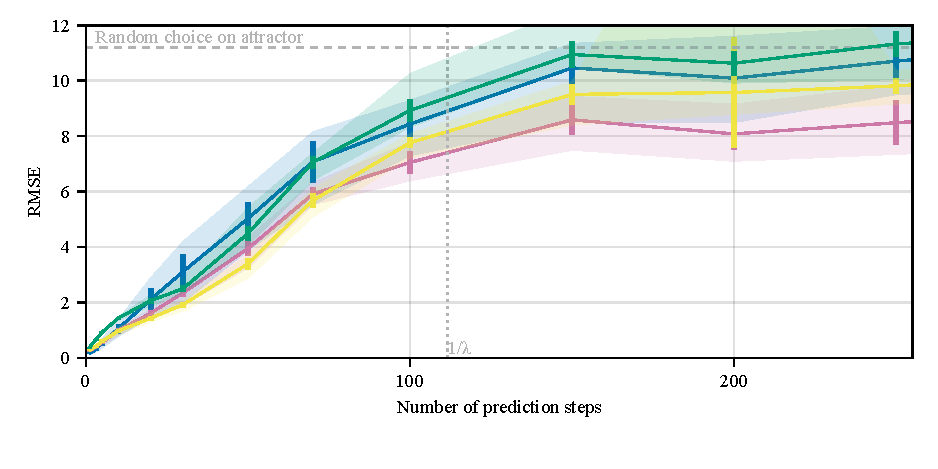
\includegraphics[width=1.1\textwidth,trim=0 8mm 0 0,clip]{../Images/OPESN/OPESN_topline_recursive_Lorenz 0_01.pdf}
        }
    \end{subfigure}

    \vspace{0.5em}

    \begin{subfigure}{\textwidth}
        \caption{Mean iterative prediction RMSE on the Lorenz series with time step size $\Delta t=0.05$ for the OPESN with delays $\tau=10,10,4$ for $m=2,3,4$ respectively, noise level $\alpha=0.1$, and total reservoir size $k\approx500$.}
        \label{fig:OPESN_iterative_0_05}
        \centering
        \makebox[\textwidth][c]{%
            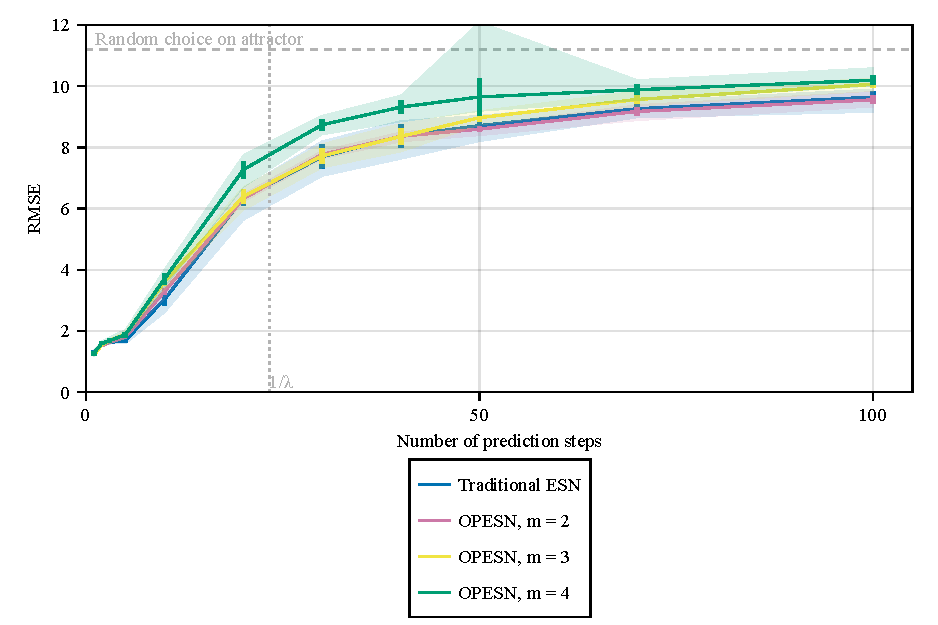
\includegraphics[width=1.1\textwidth]{../Images/OPESN/OPESN_topline_recursive_Lorenz 0_05.pdf}
        }
    \end{subfigure}

    % \caption{Mean iterative prediction RMSE for the OPESN for Lorenz x component time series with two different time steps: (a) $\Delta t=0.01$ and (b) $\Delta t=0.05$, both with additive noise $\alpha=0.1$, delay $\tau=20$ and total reservoir size $k\approx500$. The standard deviations between trials are represented by vertical bars and the range of trial results is represented by the shaded regions.}
    \caption{Mean iterative prediction RMSE for the OPESN on the Lorenz $x$ component time series with additive noise $\alpha=0.1$ and reservoir size $k\approx500$. (a) $\Delta t = 0.01$, delays $\tau=20$ for $m=2,3,4$; (b) $\Delta t = 0.05$, delays $\tau=10,10,4$ for $m=2,3,4$. Vertical bars show standard deviations; shaded regions show full range.}
    \label{fig:OPESN_iterative}
\end{figure}

\subsection{Lorenz - direct prediction}


The direct prediction results further confirm the findings that the OPESN only marginally improves upon the traditional ESN at some prediction lengths (Figure \ref{fig:OPESN_direct_0_01}). For a time step size of $\Delta t=0.01$, the traditional ESN consistently outperforms the OPESN up to 40 prediction steps. However, it is noteworthy that for 50 and 100 direct prediction steps, the OPESN with $m=2,3$ show a statistically significant (95\% CI) improvement. Additionally, the OPESN with $m=4$ shows a significantly (95\% CI) lower mean RMSE for 100 prediction steps, with the largest improvement of a mean RMSE of 6.480 ($\pm 0.035$) compared to the traditional ESN with 7.318 ($\pm 0.069$). Despite these few instances, overall the gains are marginal and do not represent a consistent advantage.


For the Lorenz time series with a time step size of $\Delta t=0.05$, the traditional ESN shows comparable or better performance than the OPESN (Figure \ref{fig:OPESN_direct_0_05}). Although, the OPESN with $m=2,3$ has a significantly (95\% CI) lower mean RMSE for 10 direct prediction steps, the gains in accuracy are marginal: The traditional ESN has a mean RMSE of 4.720 ($\pm 0.046$) compared to the OPESN $m=2$ with 4.618 ($\pm 0.036$) and $m=3$ with 4.610 ($\pm 0.037$). Overall, these results indicate that the OPESN does not provide a substantial advantage for the prediction of the Lorenz time series, and at most prediction horizons, the traditional ESN performs similarly or better.


\begin{figure}
    \centering

    \begin{subfigure}{\textwidth}
        \caption{Mean direct prediction RMSE on the Lorenz series with time step size $\Delta t=0.01$ for the OPESN with delay $\tau=20$, noise level $\alpha=0.1$, and total reservoir size $k\approx500$.}
        \label{fig:OPESN_direct_0_01}
        \centering
        \makebox[\textwidth][c]{%
            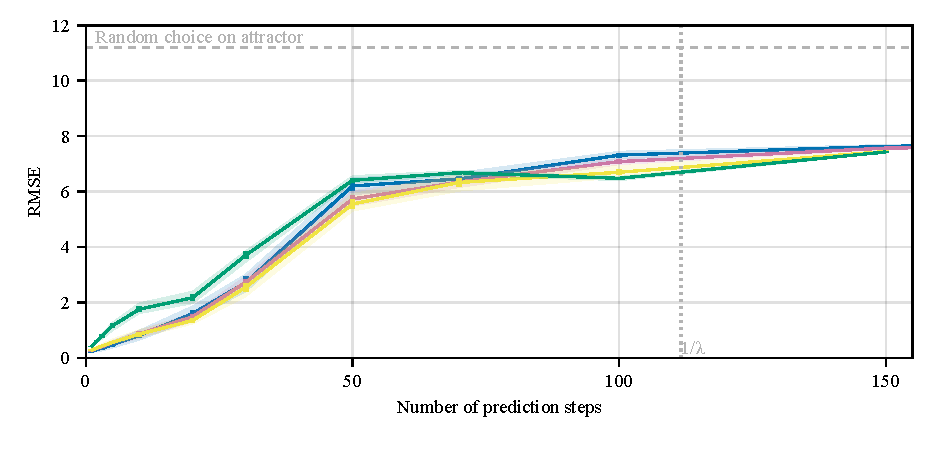
\includegraphics[width=1.1\textwidth,trim=0 8mm 0 0,clip]{../Images/OPESN/OPESN_topline_direct_Lorenz 0_01.pdf}
        }
    \end{subfigure}

    \vspace{0.5em}

    \begin{subfigure}{\textwidth}
        \caption{Mean direct prediction RMSE on the Lorenz series with time step size $\Delta t=0.05$ for the OPESN with delays $\tau=4$, noise level $\alpha=0.1$, and total reservoir size $k\approx500$.}
        \label{fig:OPESN_direct_0_05}
        \centering
        \makebox[\textwidth][c]{%
            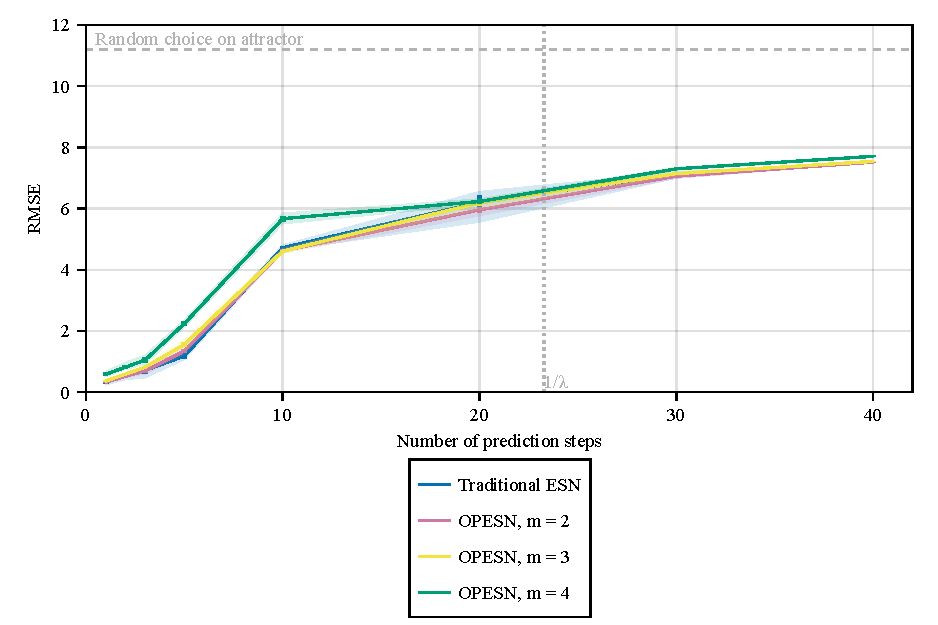
\includegraphics[width=1.1\textwidth]{../Images/OPESN/OPESN_topline_direct_Lorenz 0_05.pdf}
        }
    \end{subfigure}

    % \caption{Mean direct prediction RMSE for the OPESN for Lorenz x component time series with two different time steps: (a) $\Delta t=0.01$ and (b) $\Delta t=0.05$, both with additive noise $\alpha=0.1$, delay $\tau=20$ and total reservoir size $k\approx500$. The standard deviations between trials are represented by vertical bars and the range of trial results is represented by the shaded regions.}
    \caption{Mean direct prediction RMSE for the OPESN on the Lorenz $x$ component time series with additive noise $\alpha=0.1$ and reservoir size $k\approx500$. (a) $\Delta t = 0.01$, delays $\tau=20$ for $m=2,3,4$; (b) $\Delta t = 0.05$, delays $\tau=4$ for $m=2,3,4$. Vertical bars show standard deviations; shaded regions show full range.}
    \label{fig:OPESN_direct}
\end{figure}

\subsection{R\"ossler}

% TODO update this paragraph:
The recursive prediction results on the R\"ossler time series with time step size $\Delta t=0.1$ are plotted in Figure~\ref{fig:OPESN_rossler_iterative}.
For short prediction horizons, the OPESN tends to have higher RMSEs than the traditional ESN. However, once the prediction length reaches 10 steps, the OPESN models with $m=2,3$ begin to significantly (95\% CI) outperform the traditional ESN, with the advantage being most pronounced for $m=3$. For example, at 50 steps, the traditional ESN shows a mean RMSE of 2.234 ($\pm 0.238$) while the OPESN with $m=3$ shows a substantial improvement with a mean RMSE of 1.278 ($\pm 0.142$). The advantage ceases to be significant after 150 prediction steps.

The direct prediction results (see Figure~\ref{fig:OPESN_rossler_direct}) corroborate the advantage of the OPESN with $m=2,3$, which are significantly (95\% CI) more accurate after 30 prediction steps. While this advantage continues, the OPESN with $m=4$ only has a significant advantage between 100 and 150 prediction steps. For example, at 100 direct prediction steps, the traditional ESN has a mean RMSE of 2.075 ($\pm 0.059$), while the OPESN with $m=3$ achieves a lower mean RMSE of 1.666 ($\pm 0.037$). These results indicate that the OPESN models, particularly with $m=3$, provide a modest improvement over the traditional ESN at longer prediction lengths on the R\"ossler series.


\begin{figure}
    \centering

    \centering
    \makebox[\textwidth][c]{%
        \includegraphics[width=1.1\textwidth,trim=0 0 0 0,clip]{../Images/OPESN/OPESN_topline_recursive_rossler 0_1.pdf}
    }

    % \caption{Mean iterative prediction RMSE for the OPESN for R\"ossler $x$ component time series with time step $\Delta t=0.1$ and additive noise $\alpha=0.1$, delay $\tau=20, 20, 10$ for $m=2,3,4$ respectively and total reservoir size $k\approx500$. The standard deviations between trials are represented by vertical bars and the range of trial results is represented by the shaded regions.}
    \caption{Mean iterative prediction RMSE for the OPESN on the Rössler $x$ component time series ($\Delta t = 0.1$, $\alpha=0.1$, $k\approx500$). Delays $\tau=20,20,10$ for $m=2,3,4$, respectively. Vertical bars show standard deviations; shaded regions show full range.}
    \label{fig:OPESN_rossler_iterative}
\end{figure}

\begin{figure}

    \centering
    \makebox[\textwidth][c]{%
        \includegraphics[width=1.1\textwidth,trim=0 0 0 0,clip]{../Images/OPESN/OPESN_topline_direct_rossler 0_1.pdf}
    }

    % \caption{Mean direct prediction RMSE for the OPESN for R\"ossler $x$ component time series with time step $\Delta t=0.1$ and additive noise $\alpha=0.1$, delay $\tau=10,20,10$ for $m=2,3,4$ respectively and total reservoir size $k\approx500$. The standard deviations between trials are represented by vertical bars and the range of trial results is represented by the shaded regions.}
    \caption{Mean direct prediction RMSE for the OPESN on the Rössler $x$ component time series ($\Delta t = 0.1$, $\alpha=0.1$, $k\approx500$). Delays $\tau=10,20,10$ for $m=2,3,4$, respectively. Vertical bars show standard deviations; shaded regions show full range.}
    \label{fig:OPESN_rossler_direct}
\end{figure}

\subsection{Mackey-Glass}

The results of the OPESN prediction on the Mackey-Glass time series with time step size $\Delta t=0.5$ are shown in Figure \ref{fig:OPESN_mg_iterative}. The recursive prediction performance closely mirrors the pattern observed for the ORSESN: for short prediction horizons, the traditional ESN achieves the lowest mean RMSE, but as the prediction length increases beyond 10, the OPESN with $m=2$ and $m=3$ begin to outperform the traditional ESN. They maintain a significantly (95\% CI) lower mean RMSE than the traditional ESN for prediction lengths shorter than 50 and 70 steps, at which they lose any significant advantage.

Surprisingly, and similar to the results seen for the ORSESN, the OPESN with $m=4$ creates predictions with a substantially lower mean and standard deviation of RMSE than the other models at all prediction lengths longer than 10 steps. For example, the OPESN with $m=4$ achieves a mean RMSE of 0.060 ($\pm 0.004$) at 50 prediction steps compared to the traditional ESN with 0.208 ($\pm 0.030$), and maintains this advantage for longer prediction horizons.


\begin{figure}
    \centering

    % \begin{subfigure}{\textwidth}
    %     \caption{TODO MORE TRIALS AND LONGER TEST SERIES FOR m = 4 Mean iterative prediction RMSE on the Mackey-Glass series with time step $\Delta t=0.5$ for the OPESN with delay $\tau=20$.}
    %     \label{fig:OPESN_mg_iterative_0_5}
    %     \centering
        \makebox[\textwidth][c]{%
            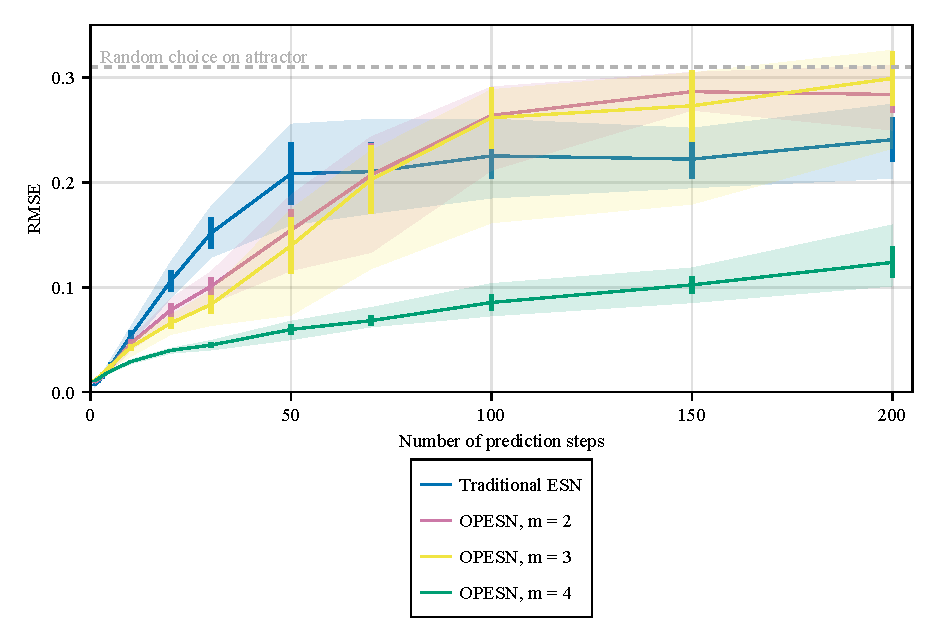
\includegraphics[width=1.1\textwidth,trim=0 0 0 0,clip]{../Images/OPESN/OPESN_topline_recursive_MG 0_5.pdf}
        }
    % \end{subfigure}

    % \vspace{0.5em}

    % \begin{subfigure}{\textwidth}
    %     \caption{TODO MORE TRIALS AND LONGER TEST SERIES Mean iterative prediction RMSE on the Mackey-Glass series with time step $\Delta t=2.5$ for the OPESN with delay $\tau=50$.}
    %     \label{fig:OPESN_mg_iterative_2_5}
    %     \centering
    %     \makebox[\textwidth][c]{%
    %         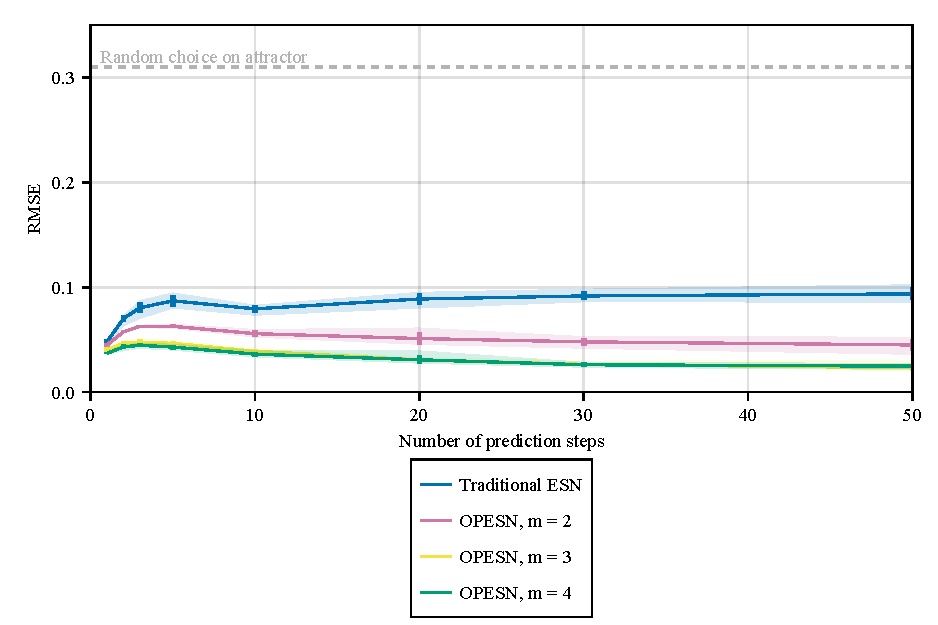
\includegraphics[width=1.1\textwidth]{../Images/OPESN/OPESN_topline_recursive_MG 2_5.pdf}
    %     }
    % \end{subfigure}

    % \caption{Mean iterative prediction RMSE for the OPESN for Mackey-Glass time series with two different time steps: (a) $\Delta t=0.5$ (delay $\tau=20$) and (b) $\Delta t=2.5$ (delay $\tau=50$), both with additive noise $\alpha=0.1$ and total reservoir size $k\approx500$. The standard deviations between trials are represented by vertical bars and the range of trial results is represented by the shaded regions.}
    % \caption{Mean iterative prediction RMSE for the OPESN for Mackey-Glass time series with $\Delta t=0.5$, delay $\tau=20$, additive noise $\alpha=0.1$ and total reservoir size $k\approx500$. The standard deviations between trials are represented by vertical bars and the range of trial results is represented by the shaded regions.}
    \caption{Mean iterative prediction RMSE for the OPESN on the Mackey-Glass time series ($\Delta t = 0.5$, $\alpha=0.1$, $k\approx500$). Delay $\tau=20$ for all $m=2,3,4$. Vertical bars show standard deviations; shaded regions show full range.}
    \label{fig:OPESN_mg_iterative}
\end{figure}

The direct prediction results for the OPESN on the Mackey-Glass system (shown in Figure \ref{fig:OPESN_mg_direct}) show a similar pattern as observed for the ORSESN: increasing the ordinal pattern dimension $m$ consistently leads to lower mean RMSE across tested prediction lengths greater than 2 steps, becoming significant (95\% CI) for 5 steps or longer. While a higher $m$ enables the OPESN to achieve improved direct predictions and mid-term iterative predictions, the $m=2,3$ models appear to suffer from instability and error accumulation in recursive prediction. By contrast, the $m=4$ OPESN appears to maintain its advantage, demonstrating stable and accurate predictions at longer horizons. Although the OPESN does not provide a substantial benefit for the Lorenz and Rossler time series, these results indicate that the OPESN can offer benefit for some attractors.

\begin{figure}
    \centering

    % \begin{subfigure}{\textwidth}
    %     \caption{Mean direct prediction RMSE on the Mackey-Glass series with time step $\Delta t=0.5$ for the OPESN with delay $\tau=20$.}
    %     \label{fig:OPESN_mg_direct_0_5}
    %     \centering
        \makebox[\textwidth][c]{%
            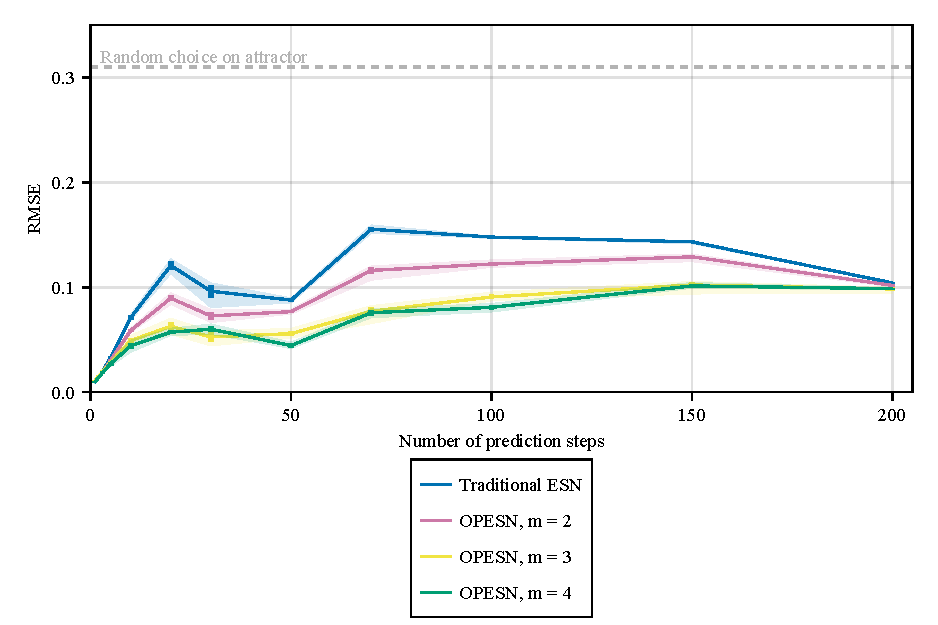
\includegraphics[width=1.1\textwidth]{../Images/OPESN/OPESN_topline_direct_MG 0_5.pdf}
        }
    % \end{subfigure}

    % \vspace{0.5em}

    % \begin{subfigure}{\textwidth}
    %     \caption{TODO MORE TRIALS AND LONGER TEST SERIES Direct prediction RMSE on the Mackey-Glass series with time step $\Delta t=2.5$ for the OPESN with delay $\tau=50,50,20$ for $m=2,3,4$ respectively.}
    %     \label{fig:OPESN_mg_direct_2_5}
    %     \centering
    %     \makebox[\textwidth][c]{%
    %         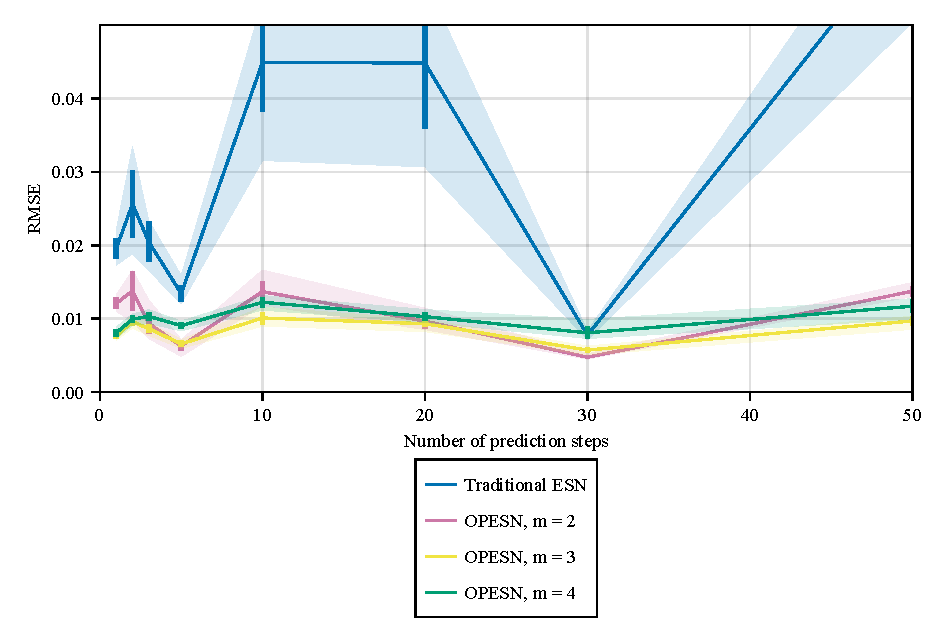
\includegraphics[width=1.1\textwidth]{../Images/OPESN/OPESN_topline_direct_MG 2_5.pdf}
    %     }
    % \end{subfigure}

    % \caption{Mean direct prediction RMSE for the OPESN for Mackey-Glass time series with two different time steps: (a) $\Delta t=0.5$ (delay $\tau=20$) and (b) $\Delta t=2.5$ (delay $\tau=50$), both with additive noise $\alpha=0.1$ and total reservoir size $k\approx500$. The standard deviations between trials are represented by vertical bars and the range of trial results is represented by the shaded regions.}
    % \caption{Mean direct prediction RMSE for the OPESN for Mackey-Glass time series with $\Delta t=0.5$, delay $\tau=20$, additive noise $\alpha=0.1$ and total reservoir size $k\approx500$. The standard deviations between trials are represented by vertical bars and the range of trial results is represented by the shaded regions.}
    \caption{Mean direct prediction RMSE for the OPESN on the Mackey-Glass time series ($\Delta t = 0.5$, $\alpha=0.1$, $k\approx500$). Delay $\tau=20$ for all $m=2,3,4$. Vertical bars show standard deviations; shaded regions show full range.}
    \label{fig:OPESN_mg_direct}
\end{figure}

\subsection{Input Routing}

The OPESN introduces two architectural features to the traditional ESN, the input routing mechanism and sub-reservoirs, and drives the input routing using ordinal partition information. Here we will test whether the improved performance - and indeed lack of improved performance - is caused by the new architectural features or the introduction of ordinal partition information. Similar to testing the gating funtion of the ORSESN, we supplied the OPESN with a random selection of sub-reservoir and compared it to the input routing driven by the ordinal partition. Figure \ref{fig:OPESN_routing_recursive_ordinal_vs_random} shows the results for the OPESN with each of $m=2,3,4$. The OPESN with random routing fails to significantly improve upon the traditional ESN at any prediction length, and in fact significantly degrades the performance for some prediction lengths - especially for the OPESN with $m=4$. We have concluded that the performance of the OPESN is likely hindered by its idiosyncratic architectural features. We can infer from this testing and the results from Chapter \ref{chap:ORSESN} that the introduction of ordinal partition information has the potential to improve model performance, however the architecture of the OPESN does not adequately exploit this potential in most cases.

\begin{figure}
    \centering

    \begin{subfigure}[t]{\textwidth}
        \caption{OPESN Input Routing - Ordinal Partition Driven vs. Random Selection, $m=2$}
        \label{fig:OPESN_routing_recursive_m_2}
        \centering
        \makebox[\textwidth][c]{%
            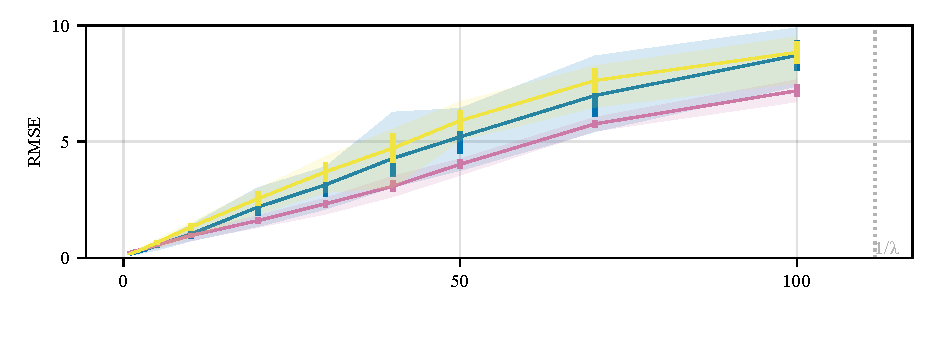
\includegraphics[width=1.1\textwidth,trim=0 6mm 0 3mm,clip]{../Images/OPESN/OPESN_routing_recursive_ordinal_vs_random_m=2.pdf}%
        }
    \end{subfigure}

    \vspace{0em}

    \begin{subfigure}[t]{\textwidth}
        \caption{OPESN Input Routing - Ordinal Partition Driven vs. Random Selection, $m=3$}
        \label{fig:OPESN_routing_recursive_m_3}
        \centering
        \makebox[\textwidth][c]{%
            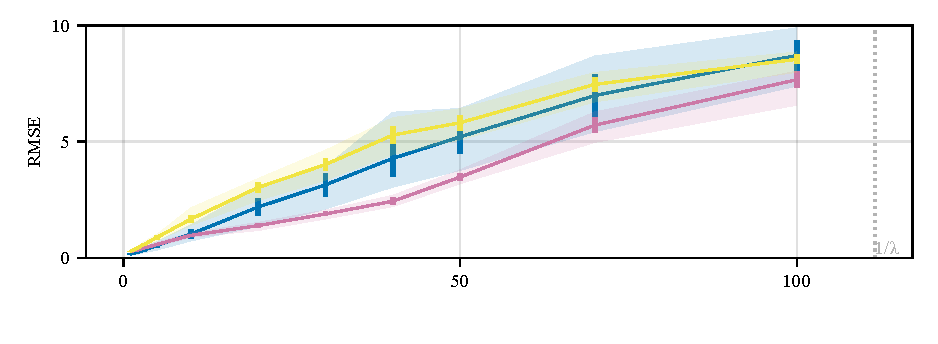
\includegraphics[width=1.1\textwidth,trim=0 6mm 0 3mm,clip]{../Images/OPESN/OPESN_routing_recursive_ordinal_vs_random_m=3.pdf}%
        }
    \end{subfigure}

    \vspace{0em}

    \begin{subfigure}[t]{\textwidth}
        \caption{OPESN Input Routing - Ordinal Partition Driven vs. Random Selection, $m=4$}
        \label{fig:OPESN_routing_recursive_m_4}
        \centering
        \makebox[\textwidth][c]{%
            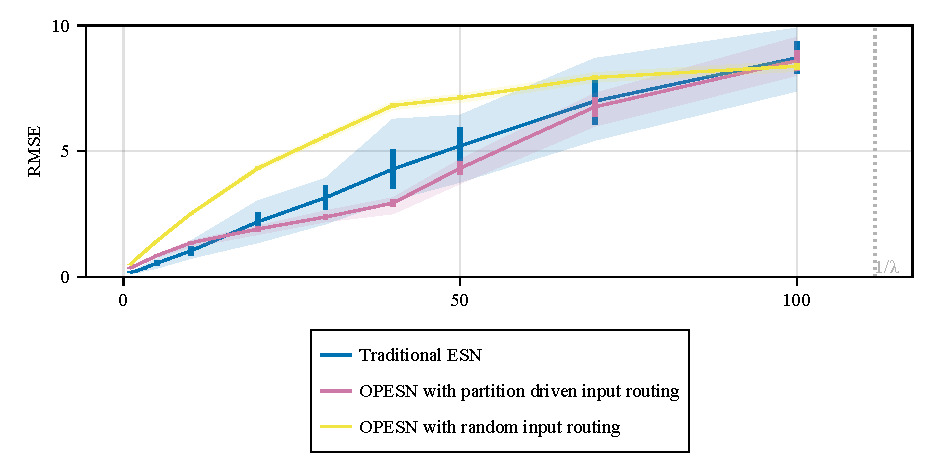
\includegraphics[width=1.1\textwidth,trim=0 0 0 3mm,clip]{../Images/OPESN/OPESN_routing_recursive_ordinal_vs_random_m=4.pdf}%
        }
    \end{subfigure}

    % \caption{Mean iterative prediction RMSE for the OPESN compared with a variant that chooses the readout randomly rather than dependent on the ordinal partition of the input, for delay $\tau=20$, noise level $\alpha=0.1$, and total reservoir size $k=468$. Subfigures (a), (b), and (c) correspond to $m=2$, $m=3$, and $m=4$, respectively. The standard deviations between trials are represented by vertical bars and the range of trial results is represented by the shaded regions.}
    \caption{Mean iterative prediction RMSE on the Lorenz $x$ component ($\Delta t=0.01$, $\alpha=0.1$, $k=468$) comparing OPESN input routing by ordinal partition versus random routing, for delays $\tau=20$ and $m=2,3,4$ in subfigures (a)-(c). Vertical bars show standard deviations; shaded regions show full range.}
    \label{fig:OPESN_routing_recursive_ordinal_vs_random}
\end{figure}

\subsection{Sub-Reservoir Connections}

As described early in this chapter, we trialed multiple methods of connecting the sub-reservoirs of the OPESN. We trialed each of these methods by finding their mean prediction RMSE across 30 trials on the Lorenz ($\Delta t = 0.01$) series. We found that no method of connection between sub-reservoirs significantly (95\% CI) improved upon the results of the disconnected sub-reservoirs. Figure \ref{fig:OPESN_recursive_sub_reservoir_connections_m_3} shows these mean prediction RMSEs for the OPESN with $m=4$, with the dashed black line representing the `disconnected sub-reservoirs' OPESN variant. As the figure illustrates, no other variant produces a significantly lower mean RMSE than the disconnected sub-reservoirs. Appendix \ref{app:sub_reservoir_connections} contains similar results for recursive and direct predictions and for OPESN models with $m=3,4$.

These results lead us to speculate that the modest advantages confered by the OPESN do not result from its modeling of an ordinal transition network, but rather from the specialisation of the sub-reservoirs akin to a mixture of experts model.

\begin{figure}
    \centering
    % ensure the graphic is centered and scaled to the text width without overflow
    \makebox[\textwidth][c]{%
        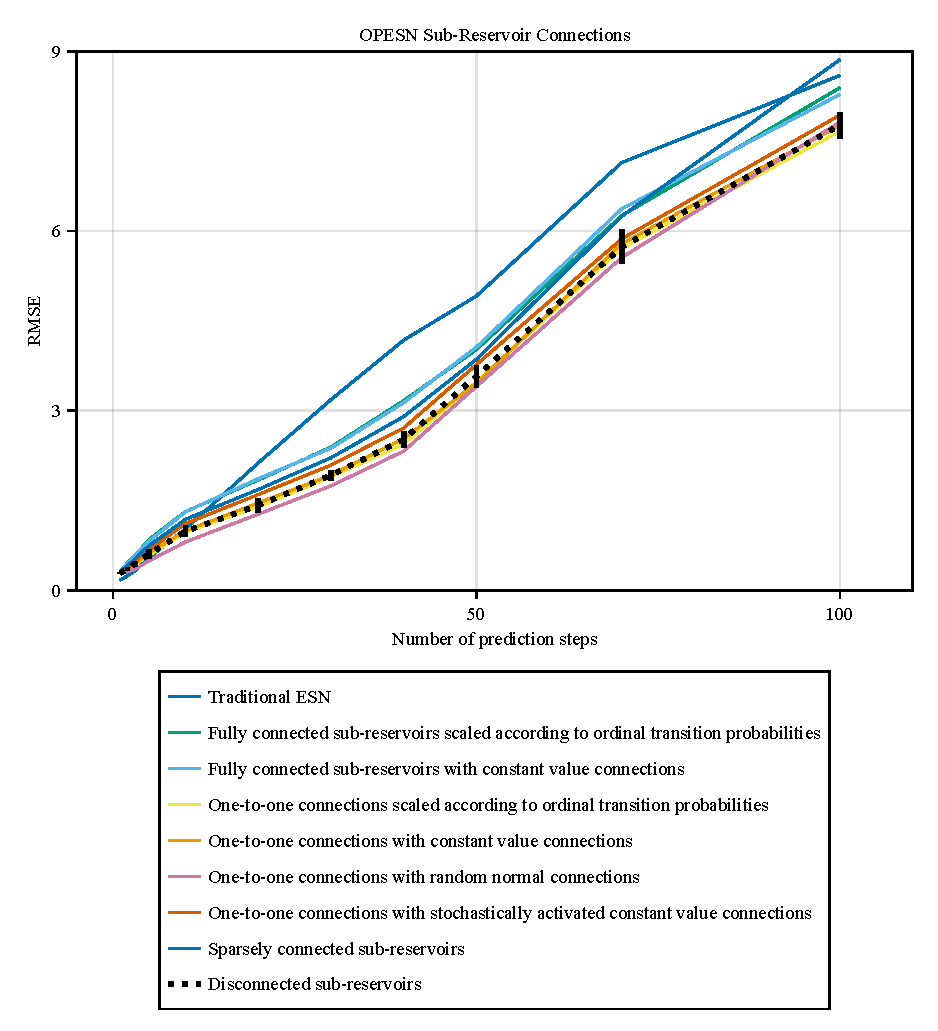
\includegraphics{../Images/OPESN/OPESN_recursive_sub_reservoir_connections_m=4.pdf}%[width=1.2\textwidth]
    }%[width=\textwidth,keepaspectratio]
    % \caption{Mean iterative prediction RMSE for the OPESN for all variants of sub-reservoir connections. Delay $\tau=20$, $m=2$, noise level $\alpha=0.1$, and total reservoir size $k=468$. The standard deviations of the trials for the disconnect sub-reservoir OPESN are represented by vertical bars.}
    \caption{Mean iterative prediction RMSE on the Lorenz $x$ component ($\Delta t=0.01$, $\alpha=0.1$, $k=468$) for OPESN variants of sub-reservoir connectivity. Delay $\tau=20$, $m=4$. Dashed black line is the disconnected baseline; vertical bars show its standard deviation.}
    \label{fig:OPESN_recursive_sub_reservoir_connections_m_3}
\end{figure}



\subsection{Resilience to Noise}

As described in Chapter \ref{chap:ORSESN}, we also tested the sensitivity of the OPESN to noise. Figure \ref{fig:OPESN_noise_resilience_direct} shows the mean direct prediction RMSE of multiple trials across values of noise $\alpha\in[0.0, 1.0]$, with four curves representing different numbers of prediction steps. As to be expected, as the level of noise increases so does the prediction RMSE for both the traditional ESN ($m=1$) and the ORSESN models ($m=2,3,4$). The noise resilience of the ORSESN models is not significantly different to the traditional ESN for direct prediction. The same noise analysis performed with iterative prediction (Figure \ref{fig:OPESN_noise_resilience_recursive}) shows the OPESN to be mildly more resilient to noise, and shows that the OPESN with $m=4$ appears to benefit greatly from the regularisation provided by additive noise. For the purposes of testing the performance of the traditional ESN and the OPESN we have chosen the `sweet spot' value of $\alpha = 0.1$, the same chosen for the ORSESN.

\begin{figure}
    \centering
    % ensure the graphic is centered and scaled to the text width without overflow
    \makebox[\textwidth][c]{%
        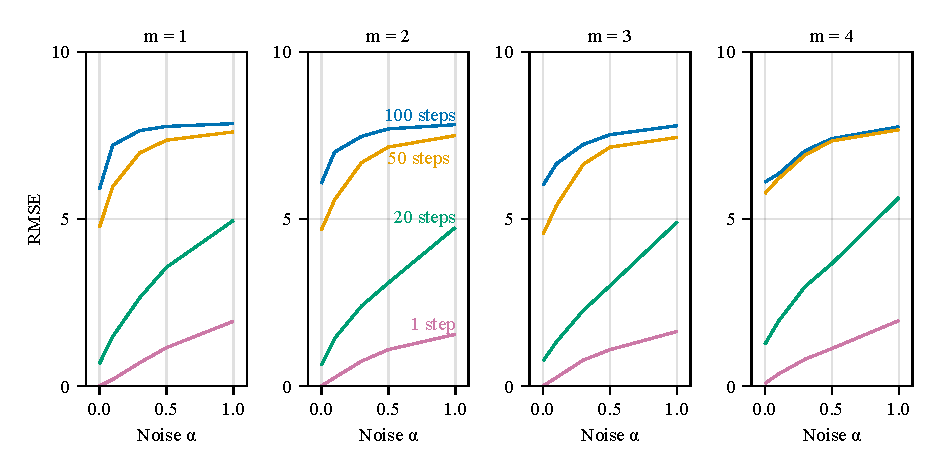
\includegraphics[width=1.1\textwidth]{../Images/OPESN/OPESN_direct_noise_resilience.pdf}%[width=1.2\textwidth]
    }%[width=\textwidth,keepaspectratio]
    % \caption{Direct prediction RMSE for the OPESN as a function of simulated data noise level $\alpha$, with delay $\tau=20$ and total reservoir size $k=468$. Curves correspond to different numbers of prediction steps, and each axis represents an OPESN with a different value for $m$. The axis labeled $m=1$ refers to the traditional ESN.}
    \caption{Mean direct prediction RMSE as a function of noise level $\alpha\in[0,1]$ for the OPESN on the Lorenz $x$ component ($\Delta t=0.01$, delay $\tau=20$, $k=468$). Curves are for lengths of prediction 1, 20, 50 and 100 steps; panels correspond to $m=1$-$4$.}
    \label{fig:OPESN_noise_resilience_direct}
\end{figure}

\begin{figure}
    \centering
    % ensure the graphic is centered and scaled to the text width without overflow
    \makebox[\textwidth][c]{%
        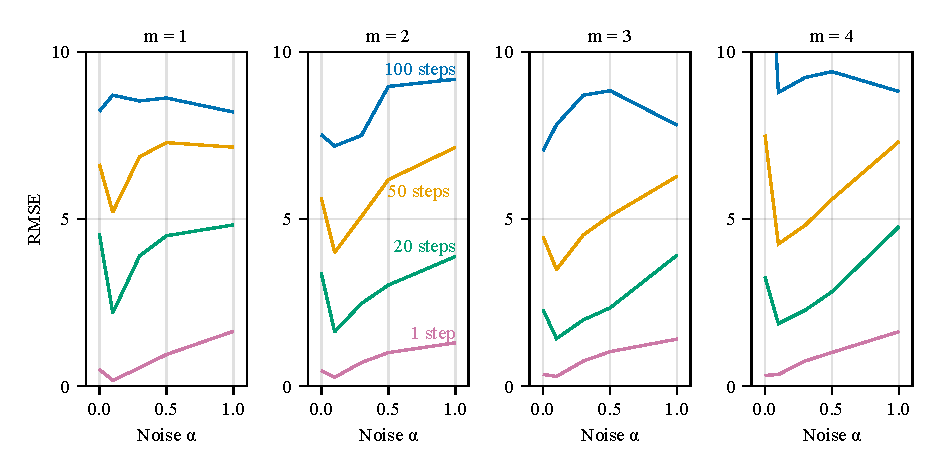
\includegraphics[width=1.1\textwidth]{../Images/OPESN/OPESN_recursive_noise_resilience.pdf}%[width=1.2\textwidth]
    }%[width=\textwidth,keepaspectratio]
    % \caption{Iterative prediction RMSE for the OPESN as a function of simulated data noise level $\alpha$, with delay $\tau=20$ and total reservoir size $k=468$. Curves correspond to different numbers of prediction steps, and each axis represents an OPESN with a different value for $m$. The axis labeled $m=1$ refers to the traditional ESN.}
    \caption{Iterative prediction RMSE as a function of noise level $\alpha\in[0,1]$ for the OPESN on the Lorenz $x$ component ($\Delta t=0.01$, delay $\tau=20$, $k=468$). Curves are for lengths of prediction 1, 20, 50 and 100 steps; panels correspond to $m=1$-$4$.}
    \label{fig:OPESN_noise_resilience_recursive}
\end{figure}



% - Multi-step


% - Single-step

% - Resilience to noise

% - Comparison across attractors

% - Effect of partition delay size

% - Other proposals

%     - Stochastic sub-reservoirs

%         - Instead of deterministic connections, connections are either activated or zeroed stochastically

%         - Depending on the transition probabilities

%     - Masking the states of the non-active sub-reservoirs before readout

%     - Internal weight matrix experiments

%         - Set connection

%         - No connecction

%         - Randomise sub-reservoir connections

%         - Make sub-reservoirs sparsely connected

%         - Self connections



    









    % Example:

    % For a $k_{layer}$ of $4$ and $3$ partitions (not actually possible).

    % \begin{center}
    % $W_{rec} = $
    % \[
    % \scalebox{0.75}{$
    % \begin{bmatrix}
    % 0.12 & 0 & 0.34 & -0.67 & 0.78 & 0 & -0.23 & 0.11 & -0.56 & 0 & 0.47 & 0 \\
    % -0.44 & 0.23 & 0 & 0 & -0.76 & 0.54 & 0 & -0.34 & 0 & 0.56 & 0.89 & 0 \\
    % 0.23 & 0.78 & 0 & 0 & 0.34 & 0.89 & 0 & 0.45 & 0.67 & 0 & -0.89 & -0.75 \\
    % 0 & 0.34 & 0.89 & 0 & 0.23 & 0 & -0.67 & 0.12 & 0 & 0.56 & 0 & -0.78 \\
    % 0.67 & 0.12 & 0 & 0.45 & 0 & 0.78 & 0 & 0.89 & 0.12 & 0 & 0.23 & 0 \\
    % 0 & 0.56 & 0.89 & 0 & 0.23 & 0 & 0.67 & 0 & 0.34 & 0.78 & 0 & 0 \\
    % 0.45 & 0 & 0.89 & 0.23 & 0 & 0.56 & 0.78 & 0 & 0.12 & 0 & 0.45 & 0.1 \\
    % 0.78 & 0.12 & 0 & 0 & 0.34 & 0 & 0.45 & 0.56 & 0 & 0.89 & 0 & 0 \\
    % 0.89 & 0.23 & 0 & 0.56 & 0 & 0.89 & 0 & 0 & 0.34 & 0 & 0.78 & 0.24 \\
    % 0.34 & 0 & 0.78 & 0 & 0.12 & 0 & 0 & 0.67 & 0 & 0.12 & 0 & 0 \\
    % 0.78 & 0.12 & 0 & 0.34 & 0 & 0.78 & 0.89 & 0 & 0.23 & 0.56 & 0 & -0.95 \\
    % 0 & 0.89 & 0.23 & 0 & 0.56 & 0 & 0.89 & 0.12 & 0 & 0.34 & 0 & 0
    % \end{bmatrix}
    % $}
    % \]
    % \end{center}
    











    % Example:
    
    % For a $k_{layer}$ of $4$ and $3$ partitions (not actually possible).

    % \begin{center}
    % $W_{rec} = $
    % \[
    % \scalebox{0.75}{$
    % \begin{bmatrix}
    % 0.12 & 0 & 0.34 & -0.67 & 0 & 0 & 0 & 0 & 0 & 0 & 0 & 0 \\
    % -0.44 & 0.23 & 0 & 0 & 0 & 0 & 0 & 0 & 0 & 0 & 0 & 0 \\
    % 0.23 & 0.78 & 0 & 0 & 0 & 0 & 0 & 0 & 0 & 0 & 0 & 0 \\
    % 0 & 0.34 & 0.89 & 0 & 0 & 0 & 0 & 0 & 0 & 0 & 0 & 0 \\
    % 0 & 0 & 0 & 0 & 0 & 0.78 & 0 & 0.89 & 0 & 0 & 0 & 0 \\
    % 0 & 0 & 0 & 0 & 0.23 & 0 & 0.67 & 0 & 0 & 0 & 0 & 0 \\
    % 0 & 0 & 0 & 0 & 0 & 0.56 & 0.78 & 0 & 0 & 0 & 0 & 0 \\
    % 0 & 0 & 0 & 0 & 0.34 & 0 & 0.45 & 0.56 & 0 & 0 & 0 & 0 \\
    % 0 & 0 & 0 & 0 & 0 & 0 & 0 & 0 & 0.34 & 0 & 0.78 & 0.24 \\
    % 0 & 0 & 0 & 0 & 0 & 0 & 0 & 0 & 0 & 0.12 & 0 & 0 \\
    % 0 & 0 & 0 & 0 & 0 & 0 & 0 & 0 & 0.23 & 0.56 & 0 & -0.95 \\
    % 0 & 0 & 0 & 0 & 0 & 0 & 0 & 0 & 0 & 0.34 & 0 & 0
    % \end{bmatrix}
    % $}
    % \]
    % \end{center}
    









    % Example:
    
    % For a $k_{layer}$ of $4$ and $3$ partitions (not actually possible).

    % \begin{center}
    % $W_{rec} = $
    % \[
    % \scalebox{0.75}{$
    % \begin{bmatrix}
    %     0.12 & 0 & 0.34 & -0.67 & 0.1 & 0 & 0 & 0 & 0.2 & 0 & 0 & 0 \\
    %     -0.44 & 0.23 & 0 & 0 & 0 & 0.1 & 0 & 0 & 0 & 0.2 & 0 & 0 \\
    %     0.23 & 0.78 & 0 & 0 & 0 & 0 & 0.1 & 0 & 0 & 0 & 0.2 & 0 \\
    %     0 & 0.34 & 0.89 & 0 & 0 & 0 & 0 & 0.1 & 0 & 0 & 0 & 0.2 \\
    %     0.9 & 0 & 0 & 0 & 0 & 0.78 & 0 & 0.89 & 0 & 0 & 0 & 0 \\
    %     0 & 0.9 & 0 & 0 & 0.23 & 0 & 0.67 & 0 & 0 & 0 & 0 & 0 \\
    %     0 & 0 & 0.9 & 0 & 0 & 0.56 & 0.78 & 0 & 0 & 0 & 0 & 0 \\
    %     0 & 0 & 0 & 0.9 & 0.34 & 0 & 0.45 & 0.56 & 0 & 0 & 0 & 0 \\
    %     0.1 & 0 & 0 & 0 & 0 & 0 & 0 & 0 & 0.34 & 0 & 0.78 & 0.24 \\
    %     0 & 0.1 & 0 & 0 & 0 & 0 & 0 & 0 & 0 & 0.12 & 0 & 0 \\
    %     0 & 0 & 0.1 & 0 & 0 & 0 & 0 & 0 & 0.23 & 0.56 & 0 & -0.95 \\
    %     0 & 0 & 0 & 0.1 & 0 & 0 & 0 & 0 & 0 & 0.34 & 0 & 0
    % \end{bmatrix}
    % $}
    % \]
    % \end{center}














